\section{Cosmology}
\subsection{Questions}
\begin{enumerate}
\item \textbf{Put on a timeline, and describe the principal events in the thermal history of the
universe, from $kT = 10$ TeV to $kT = 0.1$ eV.}
\item \textbf{Give a semi-quantitative discussion of the connection between flucuations of the
cosmic microwave background on angular scales of arcminutes to degrees, and the
baryonic structures (galaxies, clusters, correlations of galaxies) observed in the local
universe, redshift $z < 0.5$.}
\item \textbf{Which elements/isotopes are produced in Big Bang Nucleosynthesis and in what
quantities? Explain qualitatively how the yield of each depends on the cosmic baryon
density and why.}
\end{enumerate}

\subsection{The FRW Metric}
\newthought{The universe is} both homogeneous and isotropic (to at least 1 part in $10^{-5}$).
The only solutions allowed by Einstein's field equations under these assumptions is
\begin{dmath}
\d s^2 = \d t^2 - \frac{a^2(t)}{c^2}\left[\d r^2 + 
    \left\{\begin{matrix}
        r^2 \\ R^2\sin^2\frac{r}{R} \\ R^2\sinh^2\frac{r}{R} \\
    \end{matrix}\right\} \left(\d\theta^2 + \sin^2\theta\,\d\phi^2\right)\right]
\end{dmath}.
This is the Friedman-Robertson-Walker metric.  The scale-factor $a(t)$ is defined to be
1 today so that $a = 1/(1+z)$,
$r$ is the comoving distance, $R$ is the radius of curvature, and the three cases
describe a flat, closed, or open geometry respectively.

\subsection{The Friedmann Equation}
\newthought{The Friedmann equation} describes the time-evolution of the scale factor.
\begin{dgroup}
\begin{dmath}
    \dot a^2 = \frac{8}{3}\pi G\rho a^2 \mp \frac{c^2}{R^2}
\end{dmath}
\begin{dmath}\boxed{
    H^2 = H_0^2\left(\Omega_{M,0}a^{-3} + \Omega_{R,0}a^{-4} + \Omega_{\Lambda,0} + \Omega_{k,0}a^{-2}\right)
}\end{dmath}
\end{dgroup}
The second equation follows from the first by defining $H = \dot a/a$ and
$\Omega_0 = \rho_0/\rho_{c,0}$, where $\rho_c = 3H_0^2/8\pi G$ is the critical density.
The $0$ subscripts denote quantities that are measured today.

Here is a short derivation of the Friedmann equation.  Consider dynamics of a uniform sphere:

\begin{equation}
\ddot x = - \frac{GM}{x^2} = -\frac{4}{3}\pi G\rho x
\end{equation}

Since $x \sim a(t)$;
\begin{equation}
\ddot a = \frac{-4}{3}\pi G\rho a
\end{equation}

For matter, $\rho = \frac{\rho_0}{a^3}$, so $\ddot a = -\frac{4}{3}\pi G\frac{\rho_0}{a}$.  Multiply both sides by $2\dot a$ and integrate:
\begin{equation}
\int 2\dot a \ddot adt = -\frac{8}{3}\pi G\rho_0 \int \frac{\dot a dt}{a^2}
\end{equation}

So:  
\begin{equation}
\dot  a^2 =\frac{8}{3}\pi G\rho a^2 + cnst
\end{equation}

GR further tells us that the constant is $\frac{\pm c^2}{R^2}$, where R is the comoving radius of curvature.  

The Friedmann equation can be rewritted as:

\begin{equation}
H^2 = \frac{8}{3}\pi G\rho \pm \frac{c^2}{a^2R^2}
\end{equation}

So the critical density (where $R \rightarrow \infty$) is $\rho_c = \frac{3H^2}{8\pi G}$.  The universe is flat if $\rho = \rho_c$, open if $\rho < \rho_c$, and closed if $\rho > \rho_c$.

\subsection{Solutions to the Friedmann Equation}

Einstein-de Sitter model:  $\Omega = 1$, no $\Lambda$ (spatially flat, only matter).

\begin{equation}
H = \bigg(\frac{8}{3}\pi G\rho \bigg)^{0.5} = \bigg(\frac{8}{3}\pi G\rho_0 \bigg)^{0.5}a^{-1.5} = H_0a^{-1.5}
\end{equation}

\begin{equation}
a(t) = \bigg(\frac{t}{t_0}\bigg)^{\frac{2}{3}}
\end{equation}
where $t_0 = \frac{2}{3H_0}$.  

Matter and curvature model:  $\Omega \ne 1$, no $\Lambda$.

\begin{equation}
H^2 = \frac{8}{3}\pi G\rho \pm \frac{c^2}{a^2R^2}
\end{equation}
\begin{equation}
H^2 = \frac{\Omega_mH_0^2}{a^3} + \frac{\Omega_kH_0^2}{a^2}
\end{equation}

As the universe becomes large:
\begin{itemize}
\item For $\Omega < 1$, the second term dominates and the long term future is $H \sim \frac{1}{a}$, and $\dot a \rightarrow cnst$.  In this case, the universe expands forever.
\item For $\Omega > 1$, the second term is negative and H reaches 0 when $a = a_{max} = \frac{\Omega}{\Omega - 1}$.  The universe turns around ($\dot a < 0$), and ends in a Big Crunch.
\end{itemize}

Matter and $\Lambda$, flat universe.

\begin{equation}
H^2 = \frac{8}{3}\pi G\rho
\end{equation}

but here, $\rho = \rho_m + \rho_\Lambda$.  So:
\begin{equation}
H^2 = \frac{\Omega_mH_0^2}{a^3} + \Omega_\Lambda H_0^2
\end{equation}

In the far future, $\frac{\Omega_m}{a^3} \rightarrow 0$, $H \rightarrow \Omega_\Lambda^{0.5}H_0  = cnst$.  Since $H = \frac{1}{a}\frac{da}{dt}$, this means that $a \sim e^{Ht} = e^{\left(\frac{8}{3}\pi G\rho_\Lambda \right)t}$.  Thus the universe will expand exponentially.






\subsection{What Distance Means in Cosmology}
\newthought{The angular diameter distance} is the distance that is relevant for
``standard rulers''.  For an object of a known size $d$ and apparent angular size $\theta$,
the angular diameter distance is given by
\begin{dmath}\boxed{
    D_A = \frac{d}{\theta} \nolinebreak = \frac{1}{1+z} \left\{\begin{matrix}
                r \\ R\sin\frac{r}{R} \\ R\sinh\frac{r}{R} \\
            \end{matrix}\right\}
}\end{dmath}.
This is found by taking $D_A = \d l/\d\theta$ from the FRW metric.

\newthought{The luminosity distance} is relevant for ``standard candles''.  For an object of
known luminosity $L$ and observed flux $F$, the luminosity distance is
\begin{dmath}\boxed{
    D_L = \sqrt{\frac{L}{4\pi F}} \nolinebreak
        = (1+z) \left\{\begin{matrix}
                r \\ R\sin\frac{r}{R} \\ R\sinh\frac{r}{R} \\
            \end{matrix}\right\}
}\end{dmath}.
This is found by considering the surface area of a sphere with radius $r$, given by
\begin{dmath}
    A = 4\pi\left\{\begin{matrix}
            r^2 \\ R^2\sin^2\frac{r}{R} \\ R^2\sinh^2\frac{r}{R} \\
        \end{matrix}\right\}
\end{dmath},
and setting the observed luminosity to $L/(1+z)^2$ where one factor of $1/(1+z)$ is due to
the photons being red-shifted, and the other factor is due to time-dilation.\sidenote{
    To clarify a little bit, set
    \begin{dmath*}
        F = \frac{L/(1+z)^2}{A}
    \end{dmath*},
    and use the definition of $D_L$ to eliminate $F$ and $L$.
}

\subsection{Measuring Distances}\label{sec:distance_ladder}
The basic concept of distance is the distance ladder, which is basically 
different techniques used to measure distances farther and farther away.  
There is overlap between the different techniques, which allows the next 
technique to be calibrated by the previous one.  The only problem with this 
is errors and uncertainties at the bottom of the ladder propogate all the 
way up.  

The first step is parallaxes, which are reliable out to $\sim100$ pc or so.  As 
the Earth moves around the Sun, the apparent positions of stars will change 
slightly relative to more distant fixed background stars.  The distance 
to an object in parsecs is defined to be $\frac{1}{p}$ where $p$ is the 
parallax in arcseconds.  One useful trick to know for quickly converting 
between angular size and physical size- the physical size in AU of something 
$d$ parsecs away with an angular size of $\theta$ arcsec is just $\theta d$.  
So, for example, if a star and planet are $1$ pc away and are separated by 
$1$ arcsec, the planet is $1$ AU from the star.  Parallax is the only 
distance indicator that is not model dependent or reliant on some other 
calibration.  

Out to distances of $\sim1$ kpc, main sequence fitting can be used to find 
distances to main sequence stars.  If the spectral type of a star is measured, 
and the absolute magnitude of that spectral type is known from a closer 
star with a parallax distance, the difference between apparent and absolute 
magnitude gives the distance to the new star.  

This has been done for clusters of stars that contain Cepheid variables, 
leading to the next step in the distance ladder.  Cepheids are horizontal 
branch high mass stars in the instability strip of the HR diagram (see Stars 
notes).  Cepheids are useflu as distance indicators because their periods 
are tightly correlated with their luminosities by 
\begin{equation}
\log{\frac{L}{L_{\odot}}}\sim2.4+1.2\log{\frac{P}{days}}
\end{equation}
So by measuring the period of pulsation, the intrinsic luminosity can be 
determined, giving a distance.  Nearby galaxies (within $20$ Mpc) are close 
enough that individual Cepheids can be observed and used to get distances.  

Advantages:  Bright ($M_V\sim-4$ to $-7$), so the can be used in other galaxies.  
Also, we understand the physics behind their pulsation well, and can identify 
them based on their period.  

Disadvantages:  Cepheids are relatively rare since they correspond to short 
phases of stellar evolution and high masses.  Also, there are uncertainites 
about systematics of the period-luminosity relation like how it depends on 
metallicity and color.  

The tip of the red giant branch method is applicable out to similar distances 
as Cepheids.  Stars at the top of the red giant branch, right before He flash, 
have a known absolute magnitude of $-4$.  This point also corresponds to a 
drop-off in the frequency of stars, so once this is found and its brightness 
is measured, the distance can be determined.  

Advantages: Stars are bright and method is relatively precise and 
well-understood.  

Disadvantages:  Only works for old populations.  

Another method is planetary nebulae luminosity functions.  Planetary nebulae 
have an observed cut-off in luminosity at absolute magnitude $-4.5$.  The 
physics behind the cut-off is understood, and planetary nebulae can be found 
in all types of galaxies.  

For galaxies out to $\sim100$ Mpc, there are several methods to get distances, 
including the Tully-Fisher relation, globular cluster  
luminosity functions, and surface brightness fluctuations.  The Tully-Fisher 
relation is an observed correlation between the rotational velocity of 
spiral galaxies and their luminosity:
\begin{equation}
L\propto v_{rot}^4
\end{equation}
The rotational velocity is usually measured by HI $21$ cm line width.  The 
problems with this method are the relation has $\sim10-20$\% scatter, and 
the physics behind it are not well understood.  The fundamental plane gives 
similar relations for elliptical galaxies.  Globular clusters have well-defined empirical luminosity functions that can be used as 
standard candels.  Globular clusters have a peak at an absolute magnitude 
of $-6.6$.  An advantage of this method is it is not affected by dust.  
However, deep photometry is needed to measure the luminosity function, and 
this method is not as precise as others.  Surface brightness fluctuations 
involve measuring the surface brightness (flux per solid angle) in several 
regions of the same galaxy.  The observed surface brightness depends on the 
number of stars in the region, which should be similar in the different 
patches.  If the average number of stars is N, the Poisson scatter in the 
number of stars (and thus the brightness) will be $\frac{1}{\sqrt{N}}$.  
The number of stars per solid angle will also depend on distance as 
$N\propto r^2$.  So the observed scatter $\sigma\propto\frac{1}{r}$.  This 
relation can be calibrated using nearby galaxies.   

For even more distant galaxies (out to $\sim1$ Gpc), Type Ia supernovae 
can be used as standard candles to get a distance.  A tight correlation 
exists between the shape of a Ia lightcurve and the luminosity of the 
supernova, so by measuring the shape of the light curve, the distance can 
be determined.  This method is very precise, but we still don't understand 
the mechanism for a type Ia supernova.  Type Ia supernovae can be observed 
into the Hubble flow, so a plot of distance versus redshift can be used 
to determine the cosmological parameters.  The main problem with all these 
methods so far is they rely on calibrations from other methods.  One of the 
main goals of the Hubble Space Telescope was to improve these calibrations 
and determine $H_0$ more precisely.  The main focus was to better calibrate 
Cepheids and the distance to the LMC and SMC, which other methods are based 
on.  The HST $H_0$ Key Project determined $H_0=72\pm3\pm7$ km/s/Mpc.

Two methods that don't need calibration, but instead are model dependent 
are the S-Z effect (see section in Radiative) and gravitational lense 
time delays.  If a background quasar is lensed, variability in the quasar 
will be seen at different times on different sides of the lense, since the 
path length is different.  If the mass distribution of the lense is known, 
then the ratio of the path length difference to the source distance and lense 
distance can be determined.  Since the time delay is known, the path length 
difference can be calculated, giving the distance to the lense and the 
background quasar.  The modeling is very complicated however.  

\subsection{Age of the Universe}
An estimate of the age of the Universe is the Hubble time 
$t_H=1/H_0=4.4\times10^{17}h_{70}^{-1}$ s.  The exact age depends on the other 
cosmological parameters.  Other methods to get a lower limit on the age include 
globular cluster ages, white dwarf cooling times, and nucleocosmochronology 
(that's a mouthful).  Globular clusters are some of the oldest objects 
we can observe, so their ages give good lower limit to the age of the 
Universe.  The observed main sequence turnoff of a globular cluster can be 
combined with stellar isochrones to determine an age.  Uncertainties in 
the isochrone models and the distances to the clusters complicate this, 
but this methods gives lower limits ranging from around $10$ to $15$ Gyr.  
White dwarfs can also be used to age date globular clusters.  Higher 
mass stars turn into white dwarfs after only a few tens of Myr, so the 
white dwarfs will be $\sim$the same age as the cluster.  White dwarfs cool 
as they age in a fairly well understood way, so the luminosity of the 
dimmest white dwarfs in a cluster gives the age of the cluster.  There are 
still uncertainties in the cooling models though, and these white dwarfs are 
extremely faint, so this has only been done for one cluster, but the age 
agrees with the main sequence turnoff age.  Measuring abundance ratios of 
radioactive elements with Gyr or 10 Gyr half lives can also provide an estimate 
of the age.  This is difficult because the lines of these elements tend to be 
very weak in stars, but the measurements made so far give ages in the range of 
about $10-15$ Gyr.  All these methods are in agreement with the age determined 
from cosmological parameters.  

\subsection{Expansion of the Universe Tests}
Tolman Test:\newline
Observe something with a uniform surface brightness at different redshifts.  
Surface brightness is just flux per unit solid angle, so 
\begin{equation}
B=\frac{f}{d\Omega}
\end{equation}
\begin{equation}
B=\frac{L}{D_L^2}\frac{D_A^2}{dl^2}
\end{equation}
In a Euclidean, non-expanding Universe, $D_L=D_A$, so surface brightness should 
be constant for objects of constant $L/dl^2$.  In an expanding Universe, 
$D_L=D_A(1+z)^2$, so $B\propto(1+z)^{-4}$.  The intercept of the surface 
brightness scaling relations for elliptical galaxies make a good standard 
surface brightness.  Observations of clusters at different redshifts match 
$B\propto(1+z)^{-4}$.  

Hubble Diagrams:\newline
Hubble diagrams use standard candels or standard rulers to plot luminosity 
distance or angular diameter distance vs. redshift.  The shape of the 
curve gives information about the cosmological parameters.  For example, 
if the Universe has a lower density or positive $\Lambda$, it will have 
expanded faster and be larger today.  We know the Hubble constant today, 
so to slow down to this expansion rate would require more time, so the 
Universe would be older.  Since the Universe is larger, at a given 
redshift, objects would be further away, so they would look fainter and 
smaller.  A higher density Universe would behave the opposite way.  Plots 
of luminosity/angular diameter distance (or some proxy like magnitude or 
angular size) vs. redshift would show this (see Figure \ref{fig:hubble}).

\begin{figure}[!h]
\begin{center}
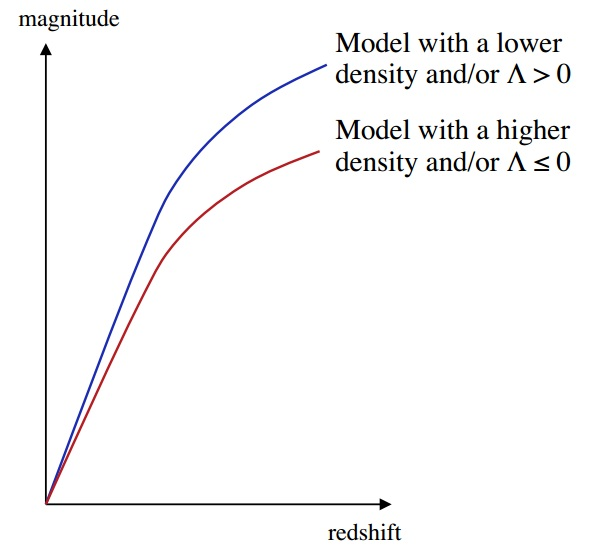
\includegraphics[width=\textwidth]{hubble.jpg}
\end{center}
\caption{A Hubble Diagram for different cosmological parameters.
\label{fig:hubble}}
\end{figure}

Early attempts at this used galaxies, clusters, and radio sources as standard 
candles and standard rulers, but galaxy and cluster evolution effects 
dominated over the effects of different cosmologies.  The use of type Ia 
supernovae (standard candles) and CMB fluctuations (standard rulers) provided 
much better tests.  

In these tests, biases from missed sources must be taken into account, as well 
as the K correction.  The idea behind the K correction is if we measure the 
light from a galaxy in a certain bandpass in our frame, the light we are seeing 
is from a bluer region of the spectrum, and this region is narrower by a 
factor of (1+z).  The bandpass emitted by the galaxy is redshifted and 
stretched when it reaches us.  This effect depends on redshift, so it must be 
taken into account when looking at galaxies at different redshifts.  The 
ratio of the flux in our frame to the flux in the galaxy's frame as a function 
of redshift has been computed for different types of galaxies and for different 
bandpasses.  

Using type Ia supernovae or CMB fluctuations indivually creates a degeneracy 
between $\Omega_{\Lambda}$ and $\Omega_M$ (here, $\Omega_M$ is density of 
baryonic and dark matter).  Combining these tests, however, breaks the 
degeneracy, and results in $\Omega_{\Lambda}\sim0.7$ and $\Omega_M\sim0.3$.

Another cosmological test is galaxy and cluster counts.  Plotting 
source counts vs magnitude (as a proxy for redshift) gives information 
on the density of the Universe.  A Universe with lower denstiy or higher 
$\Lambda$ will be larger, therefore there will be more sources to observe, 
so the curve will be higher.  A Universe with higher density will be smaller, 
and have a lower curve.  Galaxy evolution makes things difficult.  Galaxies 
were brighter in the past, so there will be extra counts at brighter 
magnitudes.  Also, because galaxies merge, there were more faint pieces in 
the past, which produces extra counts at fainter magnitudes.  To avoid this, 
really need redshifts of these galaxies.  Cluster counts rely on the 
assumption that we know what the number density of distant clusters should 
be based on the number density of nearby ones.  In a low density, older 
Universe, clusters could have formed further back in time, so we'd expect 
to see lots of distant ones.  In a higher density, younger Universe, clusters 
would only just be forming now, so we wouldn't see many distant ones.  

The combination of all these tests helps to better constrain the cosmological 
parameters and break degeneracies.  The results (I think these are pre-Planck) 
are shown in Table \ref{tab:cosmo}.

\begin{table}[H]
\centering
\begin{tabular}{c c}
\hline\hline
Parameter&Value\\
\hline
$t_0$ & $13.82\pm0.05$ Gyr\\
$H_0$ & $69$ km/s/Mpc\\
$\Omega_{baryon}$ & $0.04$\\
$\Omega_{matter}$ & $0.31$\\
$\Omega_{\Lambda}$ & $0.69$\\
\hline
\end{tabular}
\caption{Cosmological Parameters \label{tab:cosmo}}
\end{table}

\subsection{Contents of the Universe}
Baryonic Dark Matter:\newline
Observations show that the Universe's luminous matter density is only 
$\Omega_{lum}\sim0.005$, compared to $\Omega_{baryon}\sim0.04$.  This comes 
from measuring the amount of light we see, and combining this with a mass to 
light ratio.  So there is a lot of missing baryonic matter.  Two possibilities 
are massive compact halo objects (MACHOs) and cold H$_2$ gas clouds.  The most 
likely explanation looks to be warm/hot gas in galaxies groups that never 
collapsed into galaxies.  This gas would have temperatures of $\sim10^5-10^6$ 
K.  The emission from this gas would be in the far-UV/soft x-rays, which would 
be absorbed by the ISM and not be detectable.  There have been some potential 
detections through UV absorption though.  

Non-baryonic Dark Matter:\newline
This is the actual dark matter we usually talk about.  Galaxies and x-ray 
gas in clusters have typical velocity dispersions of $500-1500$ km/s, with 
cluster radii of $3-5$ Mpc.  Using the virial theorem, this gives masses 
of $10^{14}-10^{15}\ M_{\odot}$.  The total luminosity of clusters is only 
$\sim10^{12}\ L_{\odot}$, so the mass to light ratio of these clusters 
is in the hundreds.  This means lots of dark matter.  In individual galaxies, 
flat rotation curves (spirals) and flat velocity dispersions (ellipticals) 
cannot be accounted for with just the visible matter, implying the presence of 
dark matter.  The density profile of a spiral galaxy can be found by 
balancing rotation with gravity.  
\begin{equation}
\frac{v^2(r)}{r}=\frac{GM(r)}{r^2}
\end{equation}
If density is constant, then
\begin{equation}
M(r)=\frac{4}{3}\pi r^3\rho
\end{equation}
and
\begin{equation}
v(r)=r\sqrt{\frac{4\pi G\rho}{3}}
\end{equation}
This velocity profile is seen in the bulges of spirals (see Figure 
\ref{fig:vcurve}).  If the density is assumed to follow a power law
\begin{equation}
\rho(r)=\rho_0\left(\frac{r}{r_0}\right)^{-\alpha}
\end{equation}
then
\begin{equation}
v(r)=\sqrt{\frac{4\pi G\rho_0r_0^{\alpha}}{3-\alpha}}r^{1-\alpha/2}
\end{equation}
For $v(r)$ to be constant, need $\alpha=2$.  So $\rho\propto r^{-2}$ and 
$M(r)\propto r$.  This is called a singular isothermal sphere.

\begin{figure}[!h]
\begin{center}
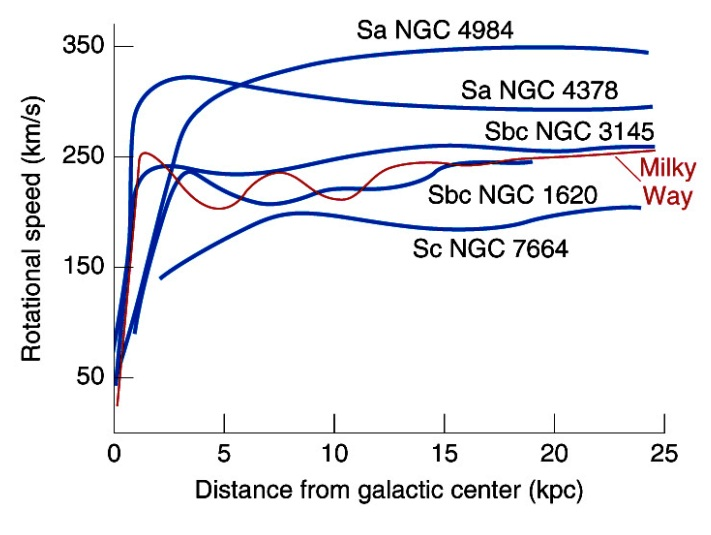
\includegraphics[width=\textwidth]{vcurve.jpg}
\end{center}
\caption{Velocity curves of spiral galaxies. \label{fig:vcurve}}
\end{figure}

Small irregular galaxies can have mass to light ratios of $100$, 
meaning they are even more dark matter dominated than big galaxies.  This is 
thought to be because the shallow gravitational potential of these galaxies 
allows the baryonic matter to be expelled, leaving only the dark matter.  

Candidates for dark matter include massive neutrinos (which we know exist, we 
just don't know how much exists), and theoretical particles like weakly 
interacting massive particles (WIMPS, not to be confused with the glorious 
society) and axions.  Modified Newtonian gravity is another, less popular 
possibility.  In terms of structure formation, dark matter is broken down into 
two classes- hot (HDM) and cold (CDM).  Hot dark matter would be relativistic 
particles such as neutrinos.  The relativistic speeds of HDM would smooth-out 
small-scale density fluctuations in the early Universe, so large structures 
would form first, and smaller structures would form later through fragmentation 
(top-down structure formation).  CDM would consist of slower moving 
particles like WIMPs or axions.  Small density fluctuations would not be 
affected, so small structures would form before large structures (bottom-up 
structure formation).  Most dark matter is probably CDM.  

Dark energy is a complete mystery.  We know the Universe's expansion is 
accelarating due to a cosmological constant $\Lambda$, with 
$\Omega_{\Lambda}\sim0.7$ (see expansion test section).  We don't know what 
dark energy actually is though.  

\subsection{Large Scale Structure}
The Milky Way is part of the local group of galaxies, which is on the edge 
of the much larger local supercluster.  The local supercluster is a $\sim60$ 
Mpc flatten group of galaxies clusters, with the Virgo cluster at its center.  
Other superclusters can be as large as $\sim100$ Mpc.  

Formation of large scale structure:\newline
For structures collapsing on a free-fall timescale, $t_{ff}\propto\rho^{-1/2}$, 
so smaller structures (which tend to be denser) form first.  For example, 
the free-fall time of a galaxy is hundreds of Myr, while for a cluster, the 
timescale is $\sim10$ Gyr.  This means galaxies should have formed early in the 
Universe (at high redshifts), and clusters should still be forming today.  This 
matches what we observe.  If the collapse of material into a cluster is 
non-spherical, the collapse will happen first along the shortest axis, forming 
a pancake.  The next shortest axis will collapse next, forming a thin 
filament.  Finally, it collapses along the remaining axis forming a spherical 
cluster.  We see these pancakes and filaments in numerical simulations and 
observations of large scale structure.  

Observations of large scale structure:\newline
Large scale structure can be mapped in 3-D using redshift surveys.  Mapping 
the positions of galaxies on the sky, then moving through different redshift 
slices reveals that the 3-D distribution of galaxies is not random.  Galaxies 
are in coherent structures.  One problem with using redshifts for this is 
the ``finger of God'' effect.  If a cluster is physically spherical, but has 
velocity dispersion amoung its galaxies, the dispersion velocities of the 
galaxies will add to or subtract from their measured redshifts, causing the 
cluster to appear elongated in redshift space (see Figure \ref{fig:finger}).  
If the cluster is still collapsing, than galaxies on the close side will 
be moving away from us with extra velocity, while galaxies on the far side 
will have extra motion towards us.  This has the effect of flattening 
the galaxy in redshift space.  

\begin{figure}[!h]
\begin{center}
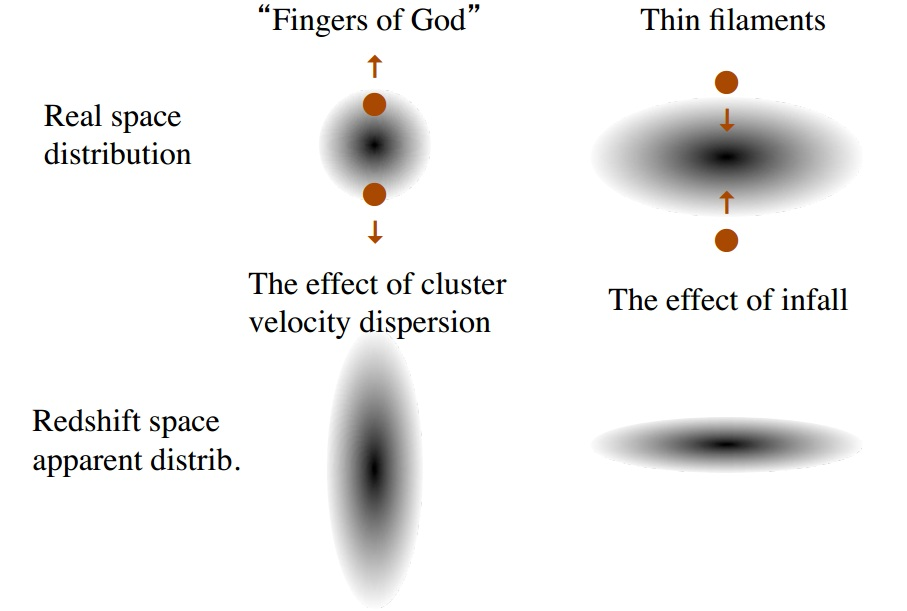
\includegraphics[width=\textwidth]{finger.jpg}
\end{center}
\caption{Velocity dispersion and infall effects on redshift maps. 
\label{fig:finger}}
\end{figure}

2 Point Correlation Function:\newline
The degree to which galaxies are clustered is quantified by the 2 point 
correlation function, $\xi (r)$.  This is defined as the excess 
probability of finding a galaxy a distance $r$ away from another galaxy, 
relative to a uniform galaxy distributin.  In other words, for a uniform 
galaxy distribution, the number of galaxies you'd expect to find a distance 
r away from a single galaxy is $dN(r)=4\pi r^2ndr$ where $n$ is the number 
density of galaxies.  If the galaxies are clustered with a correlation function 
$\xi$, then the number you would find is $dN(r)=4\pi r^2n(1+\xi(r))dr$.  
The 2 point correlation function is usually assumed to be (you guessed it!) a 
power law:
\begin{equation}
\xi(r)=\left(\frac{r}{r_0}\right)^{-\gamma}
\end{equation}
where, for galaxies, $r_0\sim5h^{-1}$ Mpc, and $\gamma\sim1.8$.  For clusters, 
clustering is stronger (clusters of clusters are more clustered than clusters 
of galaxies).  Generally, bigger structures cluster more strongly.  $\xi (r)$ 
can be estimated by counting the number of galaxy pairs in a dataset (DD) 
and by counting the number of pairs in a randomly generated uniform catalog 
(RR).  Then
\begin{equation}
\xi (r)=\frac{DD}{RR}-1
\end{equation}
There are more sophisticated methods to take into account effects at the edges 
of the dataset, but this is the basic idea.  Observations indicate that 
brigher galaxies are more strongly clustered than fainter ones, and redder 
galaxies (ellipticals) are clustered more strongly than bluer galaxies 
(spirals).  To compare with structure formation simulations, a power spectrum 
can be calculated from the Fourier transform of the correlation function.  
The observed power spectrum matches CDM simulations, and shows a peak 
corresponding to the peak in the power spectrum of CMB fluctuations (this 
isn't really explained well on the slide, but I think it has something to do 
with one of the will-ask questions).  

Peculiar Velocities:\newline
Large scale structure can also be probed using the peculiar velocities of 
galaxies.  This is a measure of their motions in addition to their Hubble 
flow velocities, in other words
\begin{equation}
v_{tot}=v_{Hub}+v_{pec}=H_0d+v_{pec}
\end{equation}
This peculiar motion is due to fluctuations in the large scale density field 
(i.e. large scale structure).  The redshifts of galaxies can be measured and 
assumed to be due to only Hubble flow.  The positions of the galaxies this 
gives can be used to find what their accelarations towards each other would 
be.  These accelarations times the Hubble time gives a peculiar velocity 
estimate.  Once the peculiar velocity has been found this way, the positions 
of the galaxies can be updated using only the Hubble contribution to their 
redshifts.  This can be repeated until things converge, giving a final density 
field.  For example, the Milky Way is falling towards the Virgo 
Cluster at $\sim300$ km/s, and the local supercluster is falling towards the 
Hydra-Centaurus Supercluster at $\sim500$ km/s.

Evolution of Clustering:\newline
Large scale structure starts out as primordial density fluctuations that 
continuously collapse under their own gravity.  Therefore, it is expected 
that clustering is stronger today than at high redshifts, since things 
will have collapsed more.  This is what is observed out to $z=1$.  At higher 
redshifts, however, clustering strength increases.  This is because the 
galaxies we see at high redshifts are a biased tracer of clustering.  
For galaxy clusters to have already formed at high redshift, they must 
correspond to higher peaks in the density fluctuations.  We see the light 
from these galaxies and clusters, but not the light from other mass that 
has not yet collapsed.  So all we can see is the few things that are most 
strongly clustered.  For example, 
at high z, the only things that have already started clustering came from 
$5\sigma$ density fluctuations.  These fluctuations collapsed quickly and are 
tightly clustered, so the clustering strenght looks high.  At lower 
redshifts, these $5\sigma$ peaks will be even more strongly clustered, 
but the total clustering strength will be brought down by $1$ and $3\sigma$ 
peaks that have finally had time to form clusters.  So clustering does 
strengthen in time, but today we see a correlation function that is brought 
down by intrinsically less strongly clustered things.  At high z, all we 
can see are intrinsically tightly clustered things.  It's like looking at 
a nearby population of stars and a far away population of stars, and concluding 
the two have different IMFs because all you can see in the distant population 
are massive stars.  

\subsection{Galaxy Clusters}
Galaxy clusters are usuallay a few Mpc across and contain $100-1000$ luminous 
galaxies and many more dwarfs.  Total masses are 
$\sim10^{14}-10^{15}\ M_{\odot}$.  Clusters are gravitationally bound, but 
not all have virialized yet.  Clusters are $\sim80$\% dark matter, $10$\% 
galaxies, and $10$\% hot x-ray gas.  Clusters are denser than galaxy groups 
and are dominated by elliptical galaxies, while groups are dominated by 
spirals.  The closest cluster to us is the Virgo cluster, $\sim3$ Mpc in size, 
$\sim16$ Mpc away, and containing $\sim2000$ galaxies, mostly dwarfs.

Finding Clusters:\newline
Cluster can be identified by finding the galaxies themselves, the x-ray gas, 
or the dark matter.  Using optical observations, overdensities of 
galaxies can be identified.  Also, color information can be used since clusters 
contain many red elliptical galaxies.  The problem with this technique is 
galaxies may appaear close together on the sky, but could be at different 
distances.  Another technique involves using the color-magnitude sequence 
for elliptical galaxies (basically a mass-metallicity relationship).  This 
sequence changes at different redshifts because of the K correction, so 
picking out galaxies along the same sequence can be used to finds ones at the 
same distance.  

The hot IGM gas in clusters can be detected by x-ray observations of thermal 
bremsstrahlung from the gas or by the S-Z effect.  Both of these techniques, 
however, are based on detecting clusters from light, not from mass.  Weak 
lensing can be used to identify the dark matter in clusters, actually detecting 
the clusters based on mass.  This is difficult to do observationally though.  

The Galaxies:\newline
Many (but not all) clusters are dominated by a large elliptical galaxy in the 
center.  The distribution of galaxies can be regular (spherically symmetric 
with increasing density toward the center) or irregular (not spherically, 
with a uniform number density, also contain more spirals).  The interpretation 
is that regular clusters are those that have had time to dynamically relax 
and reach equilibrium.  Mergers have turned the spiral galaxies into elliptical 
galaxies, and built up the large central galaxy.  Irregular clusters 
are still forming and have not come to equilibrium or used up their spirals 
yet.  

The giant elliptical galaxies in the centers of clusters are often surrounded 
by diffuse light from stars that have collected at the center of the cluster.  
These stars (originally noticed by Zwicky) have probably been 
stripped from other galaxies during mergers and have collected in the center 
of the cluster.  This is evidence that the evolution of galaxies is affected 
by their environment.  Another example is the stripping of gas from spiral 
galaxies due to the ram pressure of the IGM x-ray gas.  

The x-ray Gas:\newline
The x-ray gas in galaxy clusters has a typical temperature of $10^7-10^8$ K, 
emitting by thermal bremsstrahlung.  There is too much of this gas for it 
to have all escaped from galaxies, so it must be left over from formation of 
the cluster.  The gas was probably heated by shocks as it fell into the cluster 
potential, and since it can only cool through bremsstrahlung, it is still hot.  
The gas does contain some metals though, so some of it has been added by 
galaxies.  The temperature of the gas can be used in the virial theorem to 
find a cluster mass of $10^{14}-10^{15}\ M_{\odot}$, implying the presence of 
dark matter (see Contents of the Universe section).  The mass profile of the 
cluster can also be found using this gas (I'm not really sure how, the slide 
doesn't give much detail, but this could be used in the galaxies will-ask).  
The x-ray gas is also important for the S-Z effect for finding and determining 
distances to clusters.  As mentioned above, the x-ray gas can strip cold gas 
out of spiral galaxies in the cluster.  As expected, the most gas 
deficient spirals are located in the cores of clusters where the x-ray gas 
density is the highest.  Gas deficiency also correlates with x-ray luminosity 
(which depends on density). 

\subsection{Galaxy Relations}
Hubble Sequence:\newline
Hubble classified galaxies in a tuning fork diagram based on their appearance 
(see Figure \ref{fig:fork}).  Ellipticals are on the left, with the number 
after E corresponding to the ellipticity of the galaxy times $10$, rounded to 
the nearest integer.  The two branches on the right are for spirals with bars 
and spirals without bars.  Left to right on the branches corresponds to 
less tightly wound arms and a less prominent central bulge.  The S$0$ galaxies 
in the center are a cross between ellipticals and spirals.  They have a bulge 
and disk structure, but no spiral arms and a low star formation rate.  Hubble 
originally thought this diagram was an evolutionary sequence, so ellipticals 
are still called early type galaxies and spirals are called late type 
galaxies.  

\begin{figure}[!h]
\begin{center}
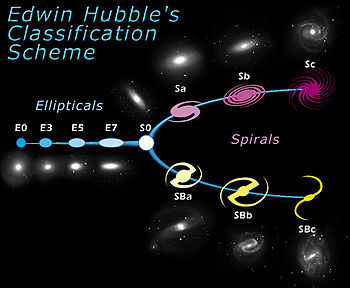
\includegraphics[width=\textwidth]{fork.jpg}
\end{center}
\caption{Hubble Sequence 
\label{fig:fork}}
\end{figure}

Hubble's classification scheme is subjective and based on appearance, not 
physics, but there are still properties that correlate with the sequence.  
Moving from left to right on the diagram, there is a transition from 
pressure support of the galaxy (kinematic pressure) to rotational support, 
an increase in star formation, red color to blue color, hot gas to cold gas 
and dust, old to still forming, and high luminosity density to low luminosity 
density.  These trends represent different star formation histories in 
ellipticals and spirals.  Ellipticals had a large burst of star formation 
early in their histories, using up all of their gas.  So all that's left is 
old, red stars.  Spirals have had a more steady star formation history, and 
are being supplied with new infalling gas (they have star formation rates of a 
few $M_{\odot}$ per year, but only a few $\times 10^9\ M_{\odot}$ of gas).  
Another difference between spirals and ellipticals is formation.  If 
ellipticals formed from the merger of stellar dominated systems, the 
dissipationless collisions would result in a pressure supported system, 
with the stars following the random $3$-D motions that they came in with.  
On the other hand, if clouds of gas merge, energy will be dissapated in the 
process, forming a disk before stars form.  

Scaling Relations:\newline
Properties of galaxies tend to follow power laws, which reflect the actual 
physics of the galaxies (even though we don't understand the physics, like 
Shri says, big galaxies are big).  Such correlations that relate distance 
dependent quantities to distance independent quantities (like the Tully-Fisher 
relation) are useful as distance indicators.  For spiral galaxies, the 
Tully-Fisher relation relates the luminosity and rotational speed of the 
galaxy:
\begin{equation}
L\propto V_{rot}^{\sim4}
\end{equation}
This relation can be hand-wavingly derived by assuming a galaxy disk has 
radius $r_d$ and uniform surface brightness $I$.  Then the total luminosity 
of the galaxy is given by $L\propto r_d^2I$.  Using the virial theorem, the 
mass inside of $r_d$ is $M\propto r_dV_{rot}^2$.  These two equations can 
be combined to give:
\begin{equation}
L\propto \left(\frac{M}{L}\right)^{-2}V_{rot}^4I^{-1}
\end{equation}
If if is assumed that all spirals have the same mass to light ratio and 
surface brighteness, then this becomes 
\begin{equation}
L\propto V_{rot}^4
\end{equation}
The surprising thing about the Tully-Fisher relation is it connects a property 
of the dark halo ($V_{rot}$) to a property of the visible matter ($L$), so 
there must some sort of feedback mechanism relating the two.  Elliptical 
galaxies follow the same proportionallity between their luminosity and 
velocity dispersion, known as the Faber-Jackson relation:
\begin{equation}
L\propto \sigma^4
\end{equation}

Fundamental Plane:\newline
Observationally, elliptical galaxies line in a plane in radius, surface 
brightness, velocity dispersion space defined by 
\begin{equation}
R\propto \sigma^{1.4}I^{-0.8}
\end{equation}
Sometimes luminosity is used instead of radius:
\begin{equation}
L\propto \sigma^{3.26}I^{-0.8}
\end{equation}
This can be approximately derived starting with the Virial Theorem
\begin{equation}
\frac{GM}{<R>}=k_E\frac{<V^2>}{2}
\end{equation}
and assuming that the observable radius, velocity dispersion, and luminosity 
(without the brackets) are related to the actual average $3$-D values (with 
the brackets) by $R=k_R<R>$, $V^2=k_V<V^2>$, and $L=k_LIR^2$.  I think all of 
these k's are just accounting for the fact that this is handwavy and 
approximate.  Solving for 
mass in the Virial Theorem and dividing by luminosity and rearranging gives:
\begin{equation}
R=K_{SR}V^2I^{-1}(M/L)^{-1}
\end{equation}
\begin{equation}
L=K_{SL}V^4I^{-1}(M/L)^{-2}
\end{equation}
with 
\begin{equation}
K_{SR}=\frac{k_E}{2Gk_Rk_Lk_V}
\end{equation}
\begin{equation}
K_{SL}=\frac{k_E^2}{4G^2k_R^2k_L^2k_V^2}
\end{equation}
The relations for $R$ and $L$ are a little off from the observed relations, 
meaning either the k's or the mass to light ratio varies with the fundamental 
plane parameters.  If lensing is used to to replace surface brightness with 
surface density, observations give 
\begin{equation}
R\propto \sigma^{1.8\pm0.2}\Sigma^{-1\pm0.2}
\end{equation}
consistent with the Virial Theorem derivation.  Looking at the fundamental 
plane with different pairs of parameters gives other relations, such as the 
Faber-Jackson relation and the Kormendy relation:
\begin{equation}
R\propto I^{-0.8}
\end{equation}
Scatter in these relations is just scatter due to the other axis of the $3$-D 
space.  

The fundamental plane is surpising because if means elliptical galaxies 
only occupy a small part of their possible parameter space, regardless of 
their formation or evolution histories.  Simulations can reproduce the plain, 
but not explain it.  

Other correlations George mentioned are the correlation between black hole 
mass and K-band absolute magnitude ($M_{BH}\propto M_K$) and the correlation 
between black hole mass and velocity dispersion ($M_{BH}\propto \sigma^{4.5}$) 
for spiral bulges and ellipticals.  These relations are not fully understood, 
but probably have to do with some sort of feedback.  

Dwarf Galaxies:\newline
Dwarf ellipticals and dwarf spheroidals are classified with regular ellipticals 
in the Hubble sequence, but follow different scaling relations.  For example, 
while regular ellipticals show decreasing average surface brightness with 
increasing total luminosity, while dwarfs follow an opposite trend.  The 
difference is the different formation and evolutionary processes for dwarf 
galaxies.  With less mass, these galaxies are less able to hold onto their gas, 
so the first generation of supernovae can blow the gas out of the galaxy, 
leaving the galaxy with a few stars and lots of dark matter.  

\subsection{Galaxy evolution}
Galaxy evolution takes two forms, evolution of stars and stellar populations 
and structural evolution of the galaxies themselves.  Structural assembly 
of galaxies through dissipationless processes is easy to model, but hard 
to observe (since it involves dark matter).  Stellar aspects of evolution are 
easy to observe, but difficult to model.  Good timescales to know for galaxy 
evolution are:
\begin{itemize}
\item $\sim100$ Myr- galaxy free-fall and cooling timescales
\item $10-100$ Myr- lifetimes of massive stars
\item $10-100$ Myr- lifetimes of AGN
\item few $100$ Myr- rotation period of a spiral galaxy
\item $\sim1$ Gyr- timescale for two galaxies to merge
\item $\sim10$ Gyr- age of Universe
\end{itemize}

Modelling Stellar Population Evolution:\newline
Assume a star formation rate as a function of time and an initial mass 
function.  Use isochrones and libraries of stellar spectra to find the 
total spectrum you'd observe from the population as a fucntion of time.  
The basic idea is since massive stars are blue, bright, and short-lived, 
different histories will produce very different looking spectra at blue 
wavelengths.  The theoretical spectra can then be matched to observations.  
Using this process, elliptical galaxies are best fit by an early burst 
of star formation followed by passive evolution with little to no star 
formation.  Spirals seem to have more gradual star formation, with a decay 
time in the star formation rate of $3-10$ Gyr.  Irregular galaxies seem to 
have constant star formation rates.  Note that observationally, star formation 
can be obscured by dust, in which case most of the energy will be reprocessed 
into the far IR and sub-mm, or unobscured, in which case the energy will be 
emitted in the UV, visible, and near IR (in both cases, what we see will be 
redshifted).  In obscured galaxies, spectra often show 2 peaks, one in the 
UV for unprocessed starlight, and a larger one (depending on how obscured the 
galaxy is) is the far IR from dust.  

Photometric Redshifts:\newline
Models can be used to predict the restframe colors of galaxies, then the 
observed colors or fluxes in different filters can be used to estimate the 
redshift (this technique is 
easier than getting spectroscopic redshifts, but not as accurate).  A similar 
technique is using continuum breaks such as the Lyman or Balmer break to 
determine redshifts.  The idea is light from the galaxy emitted at wavelengths 
shorter than $912$\AA will be absorbed by the galaxy itself or the surrounding 
IGM.  This will show up as a dropoff in intensity from the galaxy, but in our 
frame, we will see this at a redder wavelength.  By measuring the observed 
wavelength this happens at by looking at the galaxy in different filters, we 
can determine the redshift.  

Evolutionary Trends:\newline
Observations show that galaxies were smaller and brighter in the past 
(an important consideration in testing cosmology with luminosity or angular 
diameter distances).  Also, mergers were more common in the past.  The 
higher luminosities of galaxies in the past is reflected in higher surface 
brightnesses and a change in the fundamental plane for elliptical galaxies.  
Brighter galaxies have a larger increase in brightness in the past, so 
the fundamental plane actually rotates slightly.  The increase in brightness 
matches models of early bursts of star formation followed by passive 
evolution.  It is not clear if spirals were brighter in the past and how 
this affects the Tully-Fisher relation.  

Evolution in Clusters:\newline
Galaxies in clusters evolve differently than field galaxies because of 
dynamical interactions.  One example of this is the 
\emph{Butcher-Oemler effect}, that the fraction of blue galaxies in clusters 
increases dramatically at high z (I assuming faster than for the field 
population?).  Also, at a given redshift, the fraction of spiral galaxies is 
smaller for denser clusters.  \emph{Post-starburst galaxies} are a 
important product of evolution in clusters.  These galaxies show spectra 
with strong features of K and A stars, but not other features associated with 
ongoing star formation.  The interpretation is these galaxies were forming 
stars within the past $1.5$ Gyr, followed by an abrupt end to star formation.  
The general picture of this for spiral galaxies is the galaxies fall into 
the cluster at z$\sim5$, and a starburst is triggered.  The gas in the 
galaxies is stripped by the IGM, creating a post-starburst galaxy.  
Tidal interactions with other galaxies dynamically heat the disk and the 
stars slowly fade.  The result is an S0 galaxy today.  

Star Formation History:\newline
By adding up all the light from galaxies at different photometric redshifts, 
and converting this light to a star formation rate, it is possible to 
build up a star formation history of the Universe.  Star formation peaks 
at around a redshift of 3, then declines more recently and further in the past 
as galaxies were first being formed (see Figure \ref{fig:madau}).  

\begin{figure}
\begin{center}
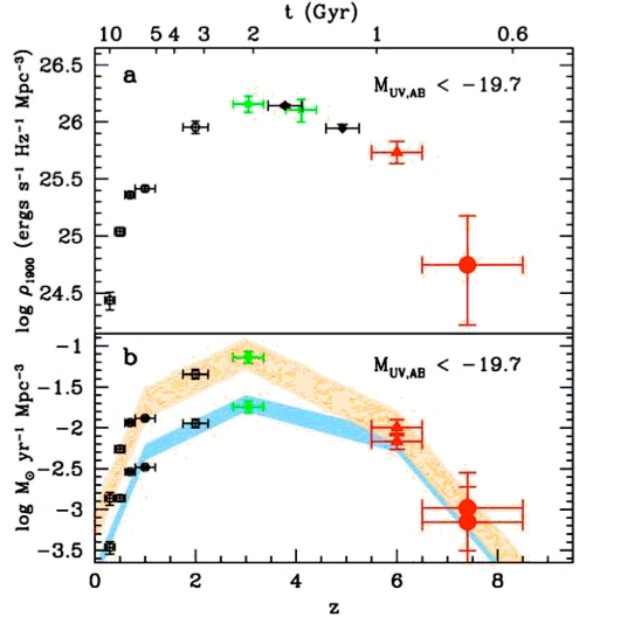
\includegraphics[width=\textwidth]{madau.jpg}
\end{center}
\caption{Flux density and star formation as a function of redshift.  I'm not 
sure what the two sequences on the lower plot are.  
\label{fig:madau}}
\end{figure}

Diffuse Backgrounds:\newline
George is on the committee, and we kept doing these sorts of problems in 
class, so we should probably review how to calculate the expected backgrounds.  
The point of these sorts of measurements is to makesure all the energy 
from different redshifts is collected (surveys for individual sources 
miss the faintest objects).  There's no redshift information though, so I'm not 
really sure what you can do with these sorts of observations (other than 
have something for students to do at teh board).  The total diffuse 
background from UV to sub-mm is $\sim100$ nW m$^{-2}$ sr$^{-1}$.  Most of 
this is in two peaks in the UV and far IR from obscured and unobscured 
galaxies.  This doesn't include the CMB, all this background at these 
wavelengths is only a few percent as bright is the CMB at its peak 
wavelengths.  

\subsection{Intergalactic Medium}
The baryons in the IGM do not belong to any individual galaxy.  Instead, 
they follow dark matter potentials, forming the ``cosmic web.''  Some of 
this gas does fall into galaxy, will gas blown out of galaxies chemically 
enriches the IGM (although the IGM still has close to primordial abundances).  
AGN and stars in galaxy provide enough flux to keep the IGM ionized (also, 
it's probably hard to recombine at IGM densities).  

One way to study the IGM is through absorption of light from background 
quasars.  Absorption systems seen this way include:
\begin{itemize}
\item Lyman $\alpha$ Forest- weak, unsaturated absorption lines implying low 
column density ($10^{14}\leq N_{HI}\leq10^{16}$ cm$^{-2}$) hydrogen clouds.  These clouds 
are spatially larger than galaxies, and have primordial metallicity.  They 
are thought to be proto-galactic clouds.  
\item Lyman Limit Systems and Damped Lyman $\alpha$ absorption lines- rare 
systems with strong H absorption lines, implying high column densities.  These 
are due to galaxies themselves or almost-formed protogalaxies.  Lyman limit 
systems have saturated Lyman $\alpha$ lines and strong absorption shortward 
of $912$\AA (similar to Lyman break galaxies).  These systems have column 
densities of $N_{HI}\geq10^17$cm$^{-2}$.  Damped Lyman $\alpha$ systems 
have column densities of $\geq10^20$ cm$^{-2}$, creating heavily saturated 
lines (more saturated than Lyman limit systems).  
\item Metal absorption lines- lines from C, Si, Mg, Al, Fe...  Mostly from 
galaxies in the line of sight.  
\end{itemize}

Gunn-Peterson Effect:\newline
The idea here is even a tiny amount of neutral H in the IGM (anything above
$x_{HI}\sim10^{-4}$) will completely absorb flux blueward of Ly$\alpha$ (does 
anyone know why Ly$\alpha$ and not the Lyman limit?).  This effect can 
be used to determine when re-ionization was completed, because if there's 
any neutral H left at a certain redshift, it will absorb all the flux from 
a background source blueward of Ly$\alpha$.  The wavelength of the dropoff 
in flux we observe gives the redshift of the H.  Observations of this effect 
show a steep dropoff in Lyman flux at redshift of around $6$, indicating that 
this was when re-ionization was complete.  

\subsection{Gravitational Lensing}
The supplementary slides of George's lecture on the IGM and lensing have some 
stuff about determining the mass profiles of galaxies from lensing.  I couldn't 
really follow what he was doing, but it might be worth looking at when we're 
practicing the galaxies will-ask question on measuring masses.  

As light from a distant source basses by a mass in the line of sight, the light 
will be bent around the mass, causing the apparent position of the source to 
change.  Assuming the impact parameter of the light $b$ is much greater than 
the Schwarchild radius of the lens, and that the light is only affected by 
the lens for a distance of order $b$, which is much smaller than any other 
distance in the problem, then the amount of deflection ($\alpha$) 
depends on $b$ and the mass of the lens:
\begin{equation}
\alpha=\frac{4GM}{c^2b}={2R_s}{b}
\end{equation}
where $R_s$ is the Schwarzchild radius.  Light rays that pass too close to the 
lens will be deflected too much and not reach the observer.  Light rays 
too far away will not be deflected enough to reach the observer.  Only 
rays within a certain range of impact parameters will be deflected to the 
observer, so the observer will see an \emph{Einstein ring} around the lens.  
If the observer, lens, and source are all along the same line, the angle 
between this line and the ring can be calculated using Figure \ref{fig:lens}.  

\begin{figure}[!h]
\begin{center}
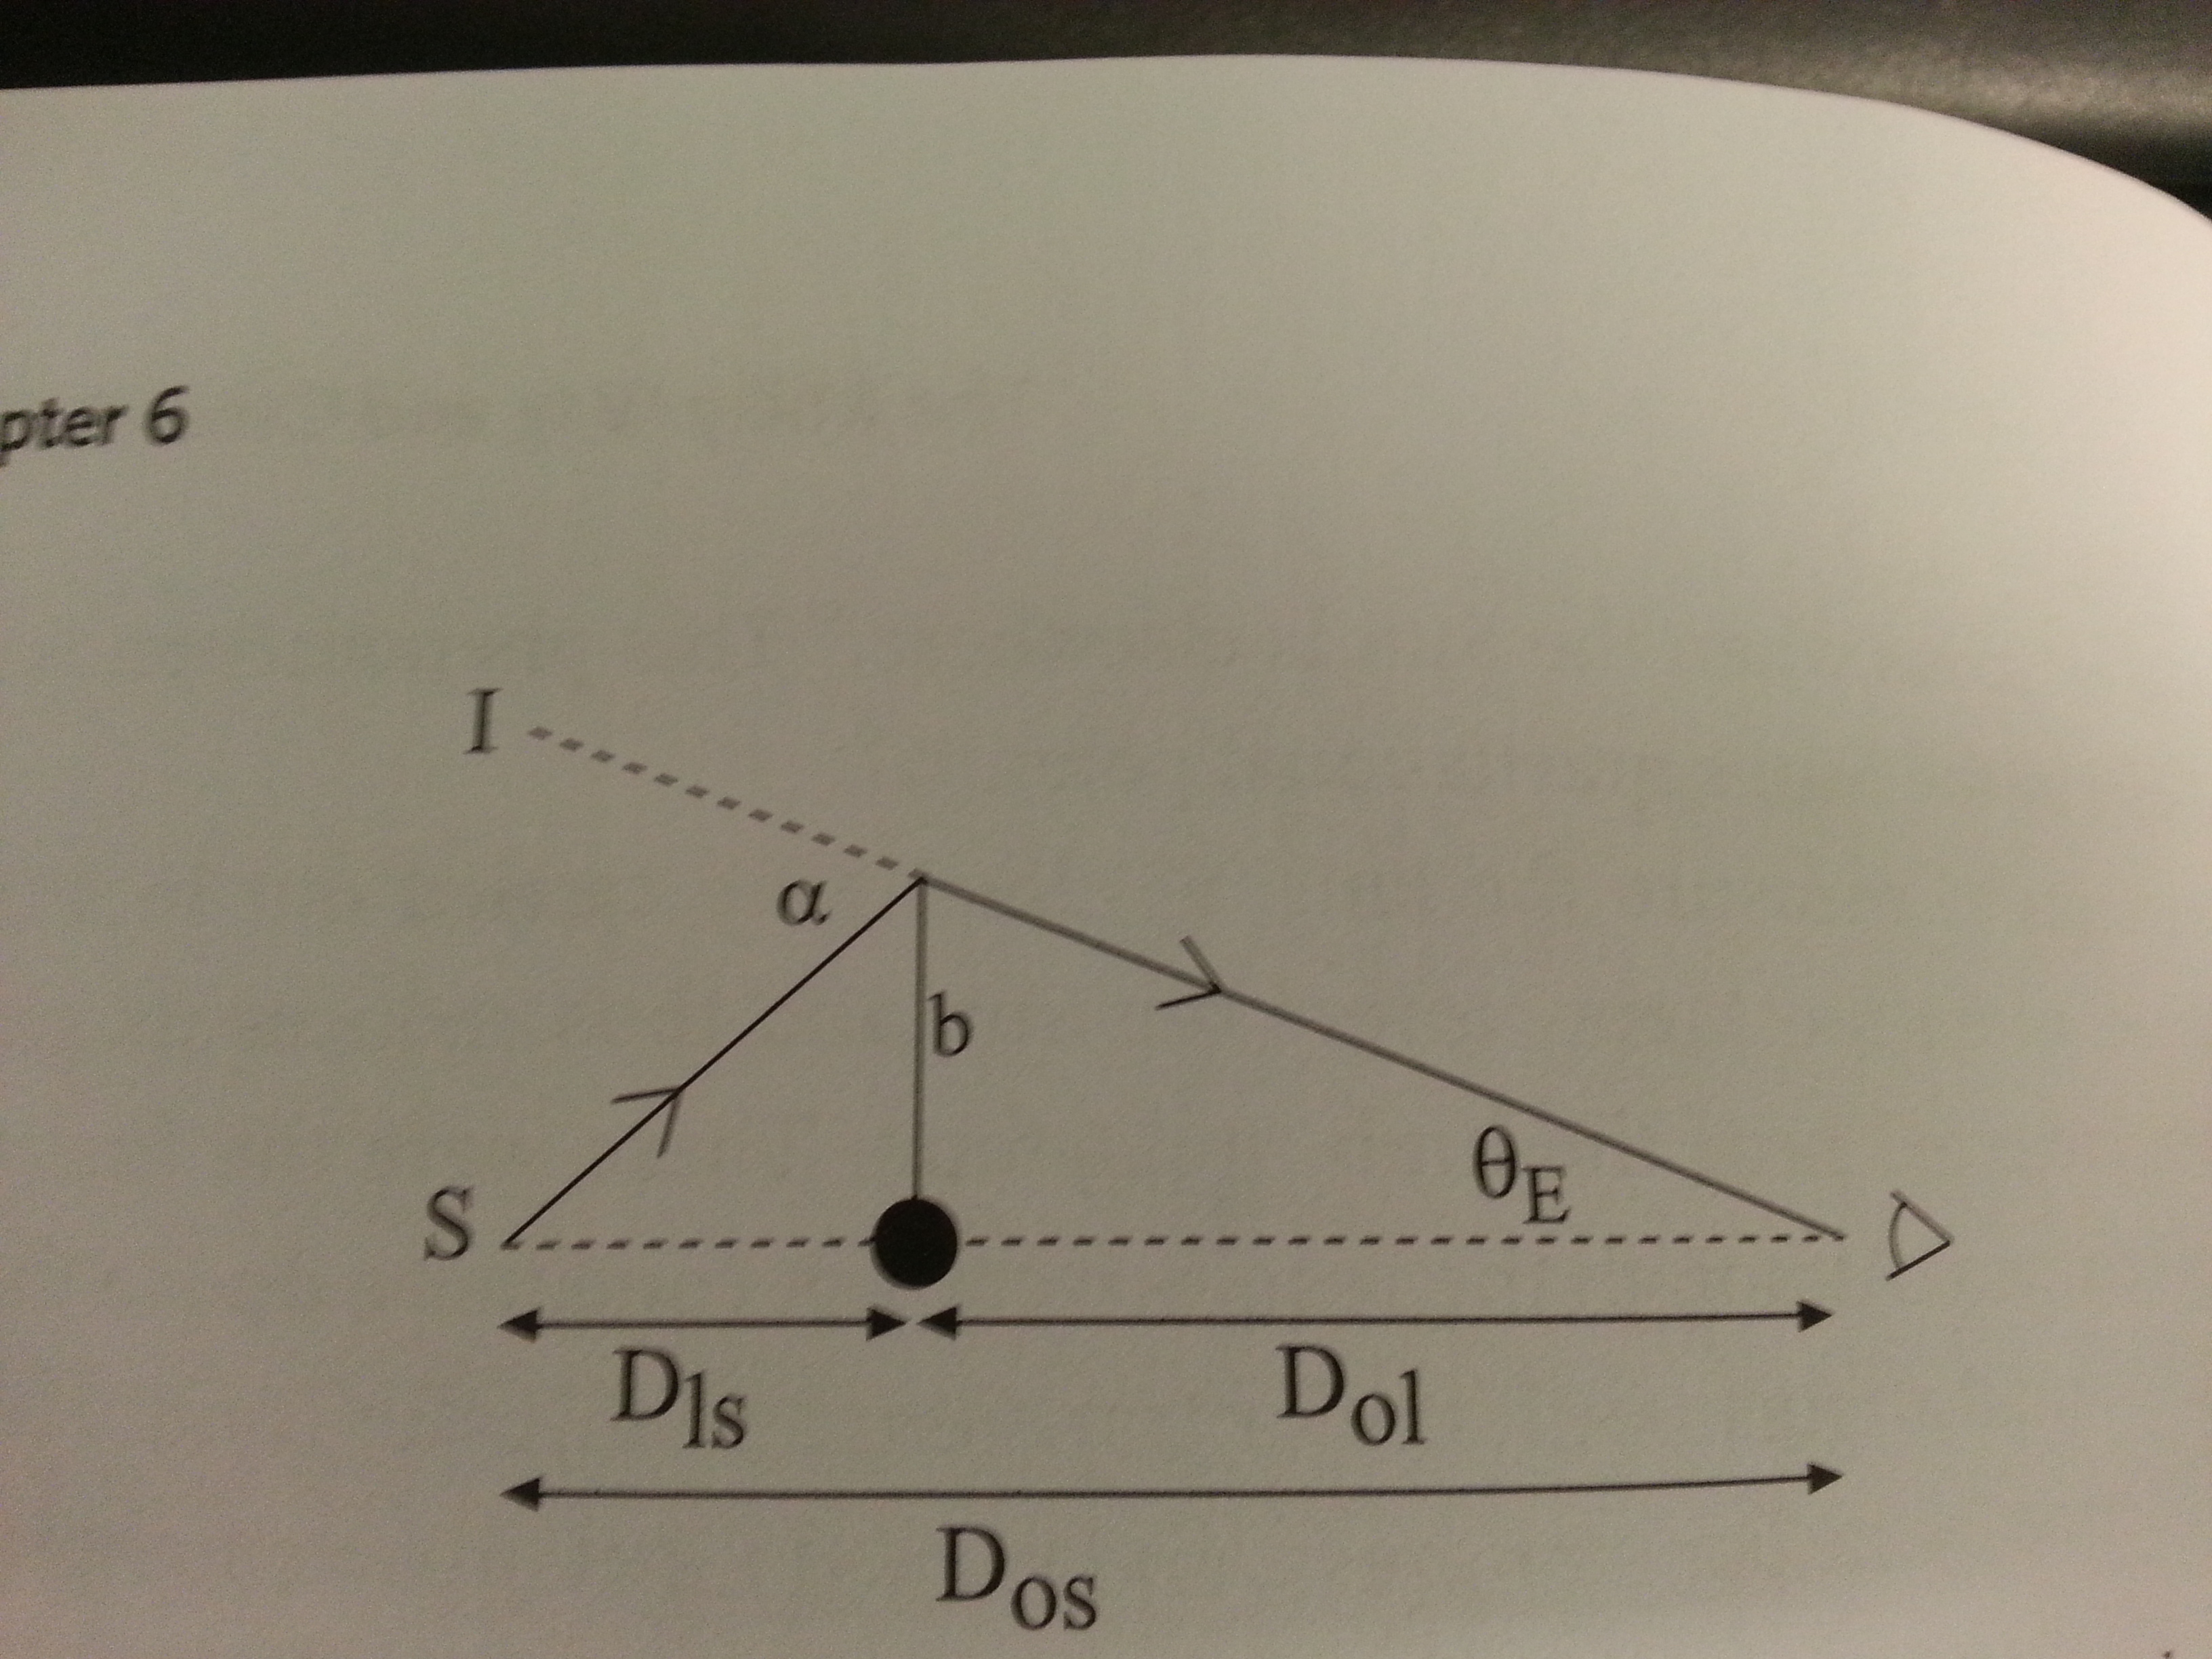
\includegraphics[width=\textwidth]{lens.jpg}
\end{center}
\caption{Gravitational lensing.  The distance from the observer to the source 
is $D_{OS}$, from the observer to the lens is $D_{OL}$, and from the lens to 
the source is $D_{LS}$.  
\label{fig:lens}}
\end{figure}

Since we are assuming $R_S/b<<1$, then $\alpha=2R_S/b<<1$.  Also, since 
$b<<D_{OL}$, $\theta_E<<1$.  With these assumptions, the distance from S to I 
is given by 
\begin{equation}
SI=\alpha D_{LS}=\theta_ED_{OS}
\end{equation}
plugging in for $\alpha$ and solving for the Einstein angle gives
\begin{equation}
\boxed{\theta_E=\left(\frac{4GM}{c^2}\frac{D_{LS}}{D_{OL}D_{OS}}\right)^{1/2}}
\end{equation}
If the source is not directly behind the lens, things are slightly more 
complicated.  The situation is shown in Figure \ref{fig:lens2}.  

\begin{figure}[!h]
\begin{center}
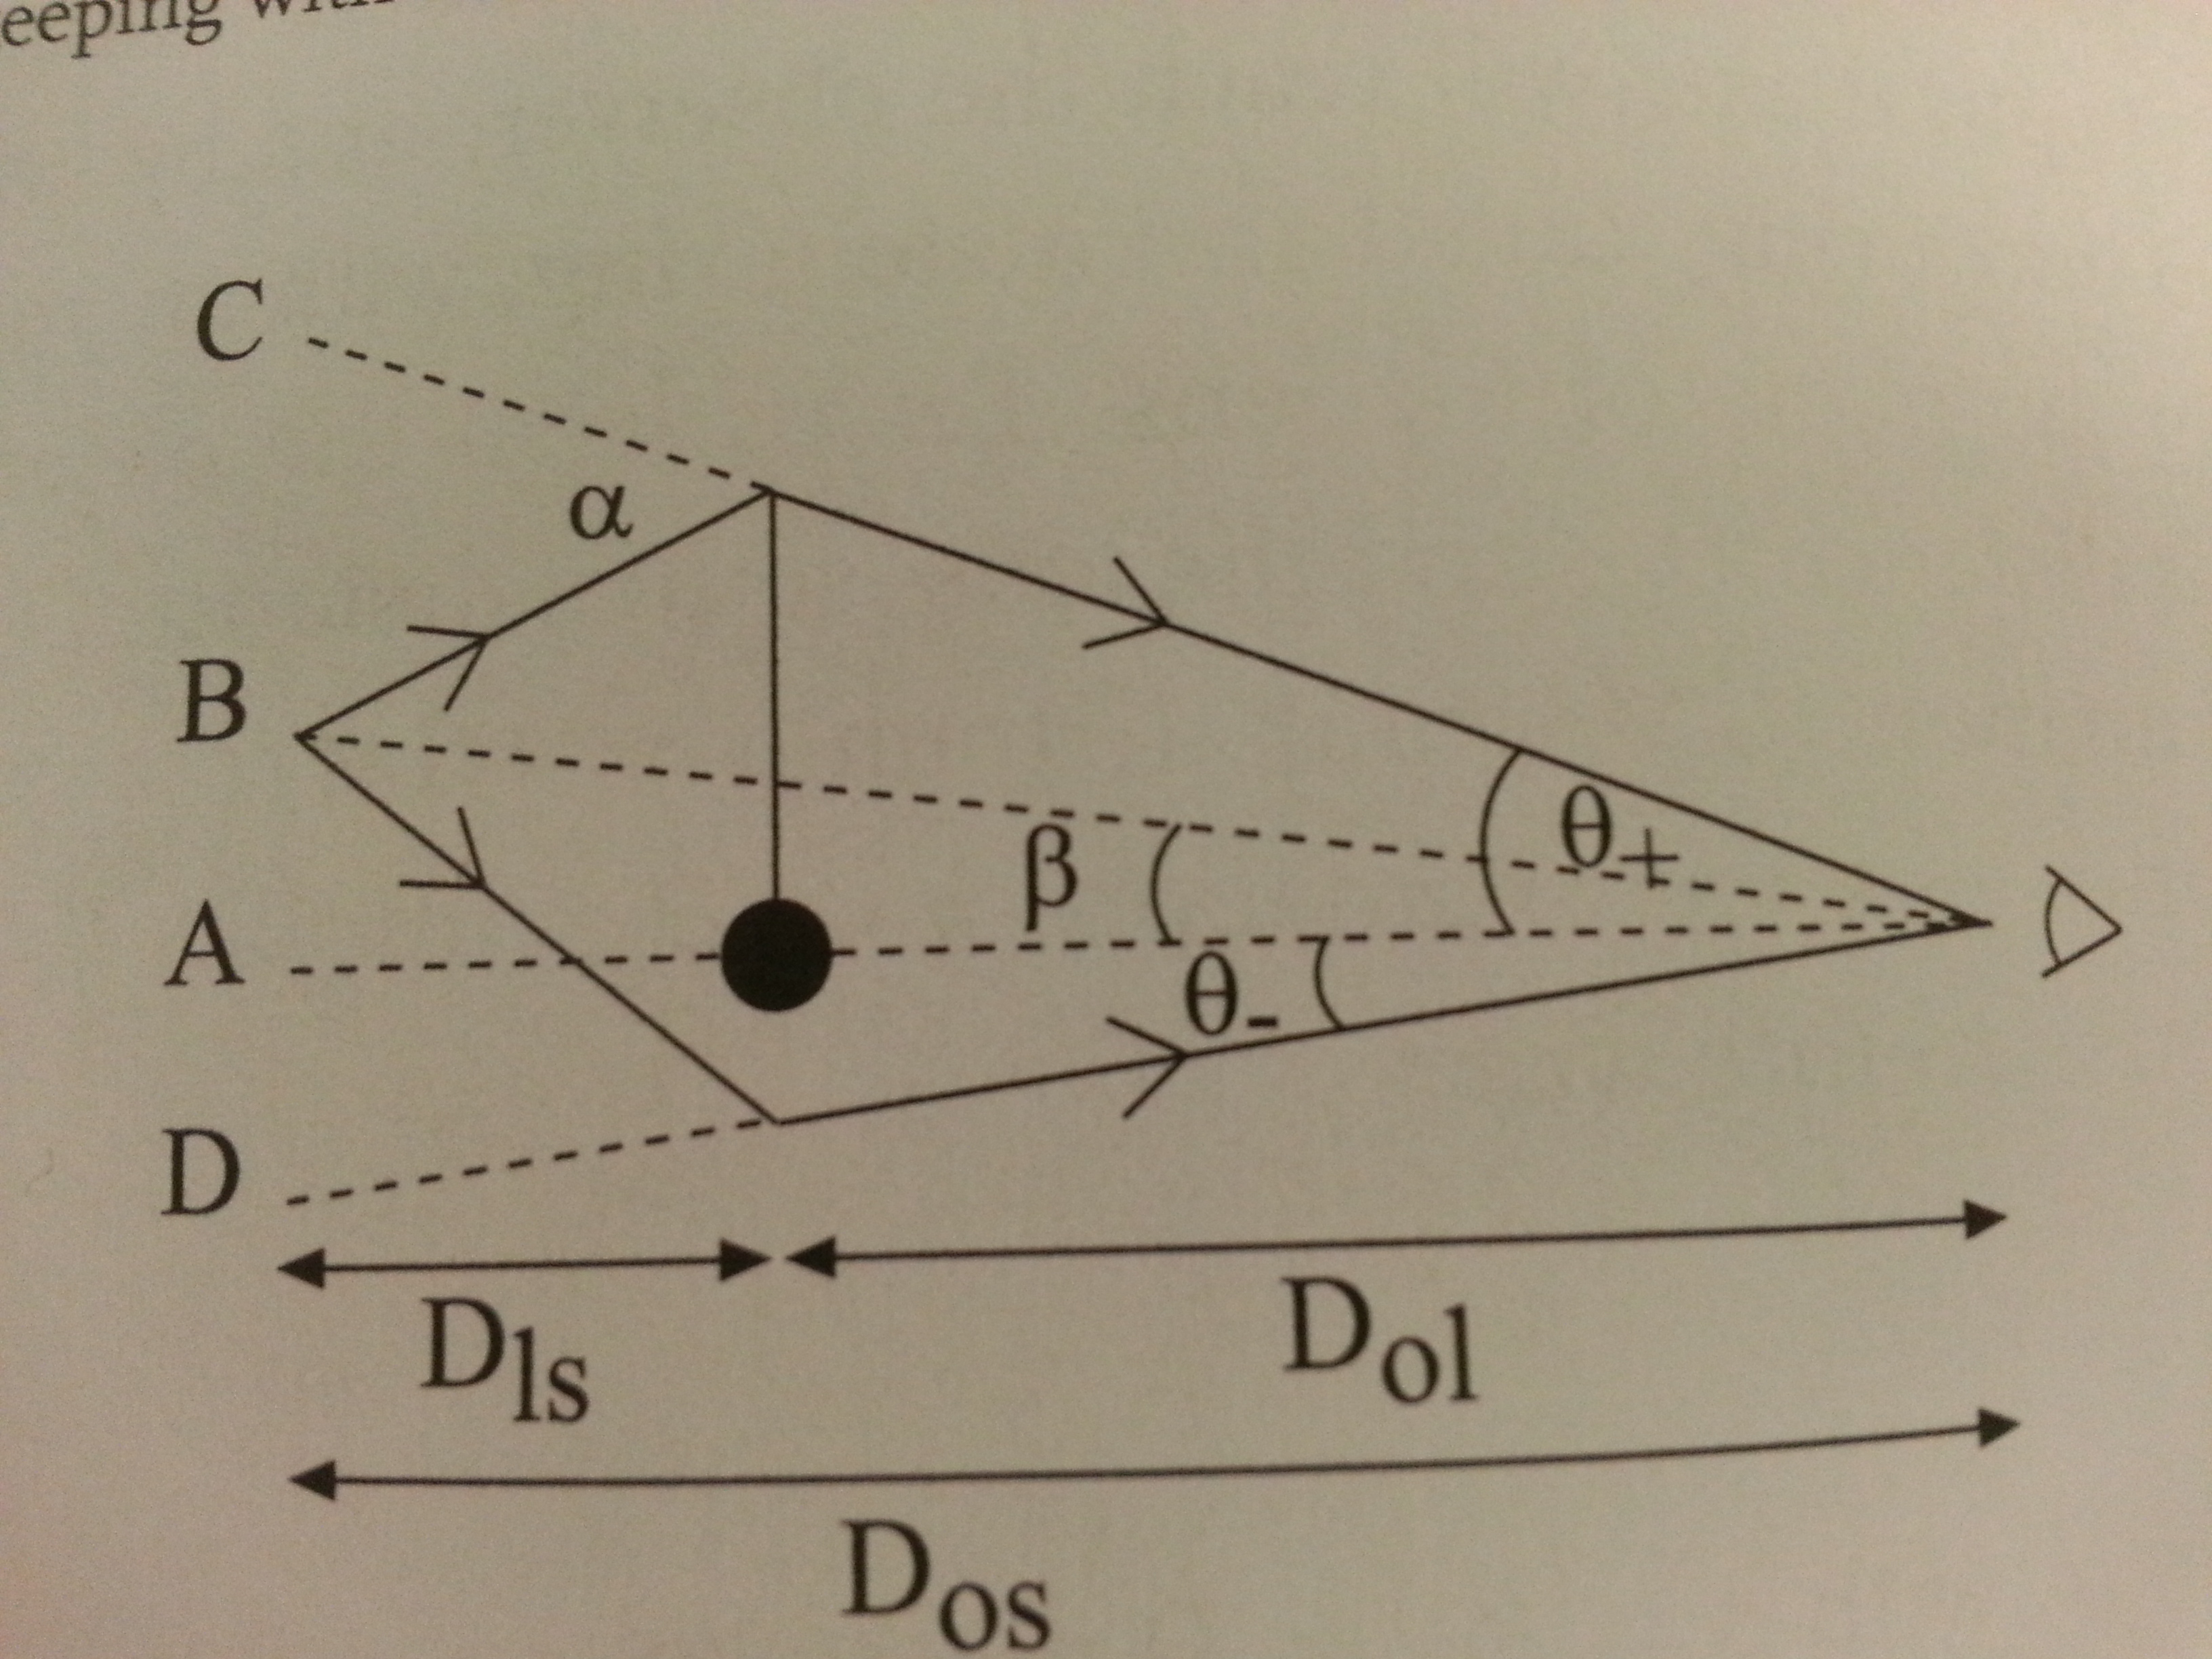
\includegraphics[width=\textwidth]{lens2.jpg}
\end{center}
\caption{Gravitational lensing with the source not directly behind the lens.  
\label{fig:lens2}}
\end{figure}

As before, the angles $\theta$, $\beta$, and $\alpha$ are small.  $\theta$ can 
be calculated by considering the length from point A to point C.  
\begin{equation}
AB+BC=AC
\end{equation}
\begin{equation}
D_{LS}\alpha+D_{OS}\beta=D_{OS}\theta
\end{equation}
Solving for $\beta$ gives
\begin{equation}
\beta=\theta-\frac{D_{LS}}{D_{OS}}\alpha=\theta-\frac{D_{LS}}{D_{OS}}\frac{4GM}{c^2D_{OL}\theta}=\theta-\frac{\theta_E^2}{\theta}
\end{equation}
This can be rewritten as a quadratic equation for $\theta$, with solution 
\begin{equation}
\theta_{\pm}=\frac{1}{2}[\beta\pm(\beta^2+4\theta_E^2)^{1/2}]
\end{equation}
Distant sources lensed by galaxy cluster give a way to measure the masses 
of the clusters, giving mass to light ratios in the hundreds.  

Gravitational lensing has also been used to test the composition of the 
dark matter in the Milky Way's halo.  If this dark matter is just dim compact 
objects (MACHOs), microlensing events would be observed when these objects 
passed into the line of sight to a star in the LMC.  A star will be lensed 
if a MACHO passes within $\theta_E$ of the line of sight to the star.  
So the cross section for lensing for a single Macho is $\theta_E^2$.  
Therefore, the probability that this Macho is currently lensing a background 
star is 
\begin{equation}
P\propto\theta_E^2\propto\left(\frac{D_{LS}}{D_{OL}D_{OS}}\right)M
\end{equation}
If a distance to the LMC and to a typical MACHO is assumed, then the 
probability of a lensing event happening at a given time from all the MACHOs 
in the halo is just proportional to the total mass in the halo.  Also, the 
duration of lensing events gives information about the mass of individual 
MACHOs.  A lensing event will last for as long as it takes the lens to 
cross the Einstein ring (in reality, it is mainly the Sun that is moving around 
the Milky Way, causing the lens to move out of alignment).  The event duration 
is then
\begin{equation}
\tau=\frac{2D_{OL}\theta_E}{v_{\odot}}=\frac{4}{v_{\odot}c}\left(\frac{GMD_{OL}D_{LS}}{D_{OS}}\right)
\end{equation}
Plugging in the distances makes the duration dependent on the mass of the 
lens, allowing the type of object doing the lensing to be constrained.  
Surveys looking for MACHOs lensing LMC stars have been conducted, finding 
typical lens masses between $0.15\,M_{\odot}$ and $0.9\,M_{\odot}$, i.e. white 
dwarfs.  The frequency of lensing events ruled out the possibility of all 
the mass in the halo being composed of MACHOs.  Also, having this many 
white dwarfs in the halo would have required a huge amount of star formation 
in the past, producing lots of metals, which we don't see.  


